\documentclass[12pt, svn, draft]{rureport}
\svnid{$Id: example-techreport.tex 48 2014-10-23 15:40:52Z foley $}
\svnidlong{$HeadURL: https://projects.cs.ru.is/svn/mechatronics/templates/techreport/example-techreport.tex $}
{$LastChangedDate: 2014-10-23 15:40:52 +0000 (fim., 23 okt. 2014) $}
{$LastChangedRevision: 48 $}
{$LastChangedBy: foley $}
% if you'd like the above information to be updated,
% use svn properties to set svn:keywords to for Id and URL (or HeadURL)
% Don't forget to set the draft to final before submitting

%% The default fixmes are:  \fxnote{} \fxwarning{} \fxerror{} \fxfatal{} (same as \fixme{})
% if you want personalized fixmes, then register the authors here
\FXRegisterAuthor{jf}{jtf}{foley}
% this registers \jfnote{}, \jfwarning{}, \jferror{}, \jffatal{}
% note the use of the two-letters 
% The three-letters are for in a fixme environment

\author{Haukur Hlíðberg, Jón Kr. Helgason, Kristófer Reykjalín, Róbert B. Ólafsson, Vladimir Omelianov,}  % My name, for the titlepage
\title{Basic Report Template}  % The title, for the titlepage
%\course{VT 1013 Hönnun}  % pick your class
%\course{T-411-MECH Mechatronics 1}
\instructor{Eyjólfur Ingi Ásgeirsson}
\graphicspath{{graphics/}{Graphics/}{./}}
%% declare the paths(s) where you graphics files can be found

\usepackage[backend=biber, bibencoding=utf8, style=ieee]{biblatex}
%\DeclareLanguageMapping{american}{american-apa}  % needed for style=apa
% If you set backend=bibtex, it will use bibtex for processing (old way)
% if you set backend=biber, you can use UTF8 characters such as Þ and ð but you will have to remember to switch from using bibtex to biber in your client
% See Chapter 7 of http://afs.rnd.ru.is/project/htgaru/trunk/how-to-get-around-projects.pdf 
% If you just want to use bibtex directly without using BibLaTeX, then comment out the line.
\addbibresource{references.bib}

\usepackage[final,hidelinks]{hyperref} % must be last package loaded
% it makes hyper-references (citations, URLs, etc) clickable

\begin{document} % this tells the compiler that it is time to make
                 % text to print instead of just getting ready.
\maketitle  % make a title page from the Title, Date, and Author

%\section*{Errata} %%section* avoids putting a number 


\section{Inngangur} % sections break up the document into pieces

Í þessu verkefni áttu nemendur að setja fram rannsóknarspurningar sem þeir gætu svarað með gögnum frá Hagstofu Íslands. Fyrst var spurt, hvað er það sem okkur finnst áhugavert, þar sem við allir eru nemendur við Háskóla Reykjavíkur þá fannst okkur tilvalið að fjalla um  menntun og laun ýmissia starfsstétta.Skoðað var meðaltal heildarlauna starfstétta og eftir þær niðurstöður skoðuðum við meðaltalsvinnustundir á milli kynja milli ára,  hvernig menntunargráða ýmissa aldurshópa skiptist niður á milli ára, skoðum kynjahlutfall háskólagráða innan höfuðborgarsvæðis og utan þess.//
Í þessu verkefni áttu nemendur að setja fram rannsóknarspurningar sem þeir gætu svarað með gögnum frá Hagstofu Íslands. Fyrst var spurt, hvað er það sem okkur finnst áhugavert, þar sem við allir eru nemendur við Háskóla Reykjavíkur þá fannst okkur tilvalið að fjalla um  menntun og laun ýmissia starfsstétta.// 

Skoðað var meðaltal heildarlauna starfstétta og eftir þær niðurstöður skoðuðum við meðaltalsvinnustundir á milli kynja milli ára,  hvernig menntunargráða ýmissa aldurshópa skiptist niður á milli ára, skoðum kynjahlutfall háskólagráða innan höfuðborgarsvæðis og utan þess.// 

=======
Í þessu verkefni áttu nemendur að setja fram rannsóknarspurningar sem þeir gætu svarað með gögnum frá Hagstofu Íslands. Fyrst var spurt, hvað er það sem okkur finnst áhugavert, þar sem við allir eru nemendur við Háskóla Reykjavíkur þá fannst okkur tilvalið að fjalla um  menntun og laun ýmissia starfsstétta.\\ 

Skoðað var meðaltal heildarlauna starfstétta og eftir þær niðurstöður skoðuðum við meðaltalsvinnustundir á milli kynja milli ára,  hvernig menntunargráða ýmissa aldurshópa skiptist niður á milli ára, skoðum kynjahlutfall háskólagráða innan höfuðborgarsvæðis og utan þess.// 

>>>>>>> .r116
Gögnin sem voru fengin voru þannig að hægt var að svara mörgum spurningum og túlka á margan hátt, aðalega vildum við sjá hvernig menntun og laun dreifðist á milli kynja og svo útfrá þeim spurningum var hægt að spyrja sig að enn fleiri spurningum eins og nefnt er að ofan.


% Áður en hafist var handa byrjuðum við að setja fram nokkuð opnar spurningar sem snérust að menntun, menntunnar stigum, launum fyrir mismunandi aldurshópa og hvort mætti finna eitthverja fylgni í þessum gögnum.



\section{Framkvæmd}

Þegar búið var að velja hvaða gögn(csv skrár) við myndum koma til að með að nota byrjaði einn hópmeðlimur(K.R.Þ.) að forvinna gögnina í python sem myndi einfalda vinnuna fyrir alla og þar með tíma. Inni í þessari forvinnu var meðal annars settar inn í viðeigandi breytur, prentaður út listi með öllum lykil heitum á breytum(keys). Eftir það settist hópurinn niður og skrifaði spurningar sem okkur fannst áhugaverða og líklegt að það kæmi spennandi niðurstöður úr.//

Forritunnar vinnan gat þá hafist og tóku allir meðlimir hópsins að sér 1-3 spurningar og skrifuðu kóða fyrir þær. Þegar allir voru orðnir sáttir við sínar niðurstöður voru gerð föll fyrir hvern og einn kóða sem skiluðu viðeigandi niðurstöðum og var ein yfirskrá gerð sem er keyrð og birtir allar niðurstöðurnar, í þessu tilfelli línu og súlurit sem birt eru í kafla\ref{nidurstodur} hér að neðan.

\section{Aðferðir}

Aðferðafræðin sem var sett á hópfundi, eftir að einn hóp meðlimur (Team leader Krillvélin) var búinn að forvinna gögin, að allir myndu velja spurningu/ar og vinna úr gögnunum og búa til sinn eigin kóða í Python. Síðan voru gögnin borin saman svo hægt væri að rýna í niðurstöðurnar og svara sem flestum spurningum og hvort væri hægt að draga einhverjar niðurstöður úr þeim niðurstöðum sem fengust.

Uppbygging kóðanna er mjög svipuð þótt hver og einn gerði sinn eiginn kóða, það er byrjað á því að taka inn allar þær 
 
%Sú aðferðar fræði var tekinn í pólinn að allir í hópnum myndu vinna sinn eiginn kóða, en á 3 tíma fresti væru teknar tíu mínótur



\section{Niðurstöður}\label{nidurstodur}
%vladimir
Á mynd [\ref{fig:menntunall}]við getum séð að mest fjöldi af menntað fólk á íslandi eru á bili 30 og 49 ára, næst algengasta aldurs hóp er 50 til 64 ára.
Áhugavert að sjá hvernig fjöldi að mentaðu fólk skiptist á milli kyn, menntun og aldrusflókk. Til dæmis:
\begin{itemize}  
	
	\item Breytinging hjá konum meðgrunnmentun í sem gerðist í  2008 þar sem konur í aldrusflokki 50 - 64 ára eru fleiri en  en 30 - 49 ára eins og sérs á mynd [\ref{fig:menntungrunn}]
	
	\item Það eru mun fleira Karlmen með háskólamentun en konur skv. mynd [\ref{fig:menntunhs}], en það virðist vera fleira og fleira konur sem eru að detta í 30 - 49 ára flokk.
	
	\item Það er minni bil milli aldurs flokkum 30 til 49 og 50 til 69 ára hjá baðum kynum,
	og fljöldi að konum men Starf og framhandsmenntun er mjög svipað á milli aldrusflokka 20 til 24 og 50 til 64 ára, miðað við karla skv mynd [\ref{fig:menntunfram}] 
	
	\item Einhvern hlut að vegna það vantar upplýsingar um menntun hjá fleira Körlum en konum skv mynd [\ref{fig:menntunvantar}]
	
\end{itemize}



\subsection{Kynjahlutfall vinnustunda}

\begin{figure}
	\centering 
	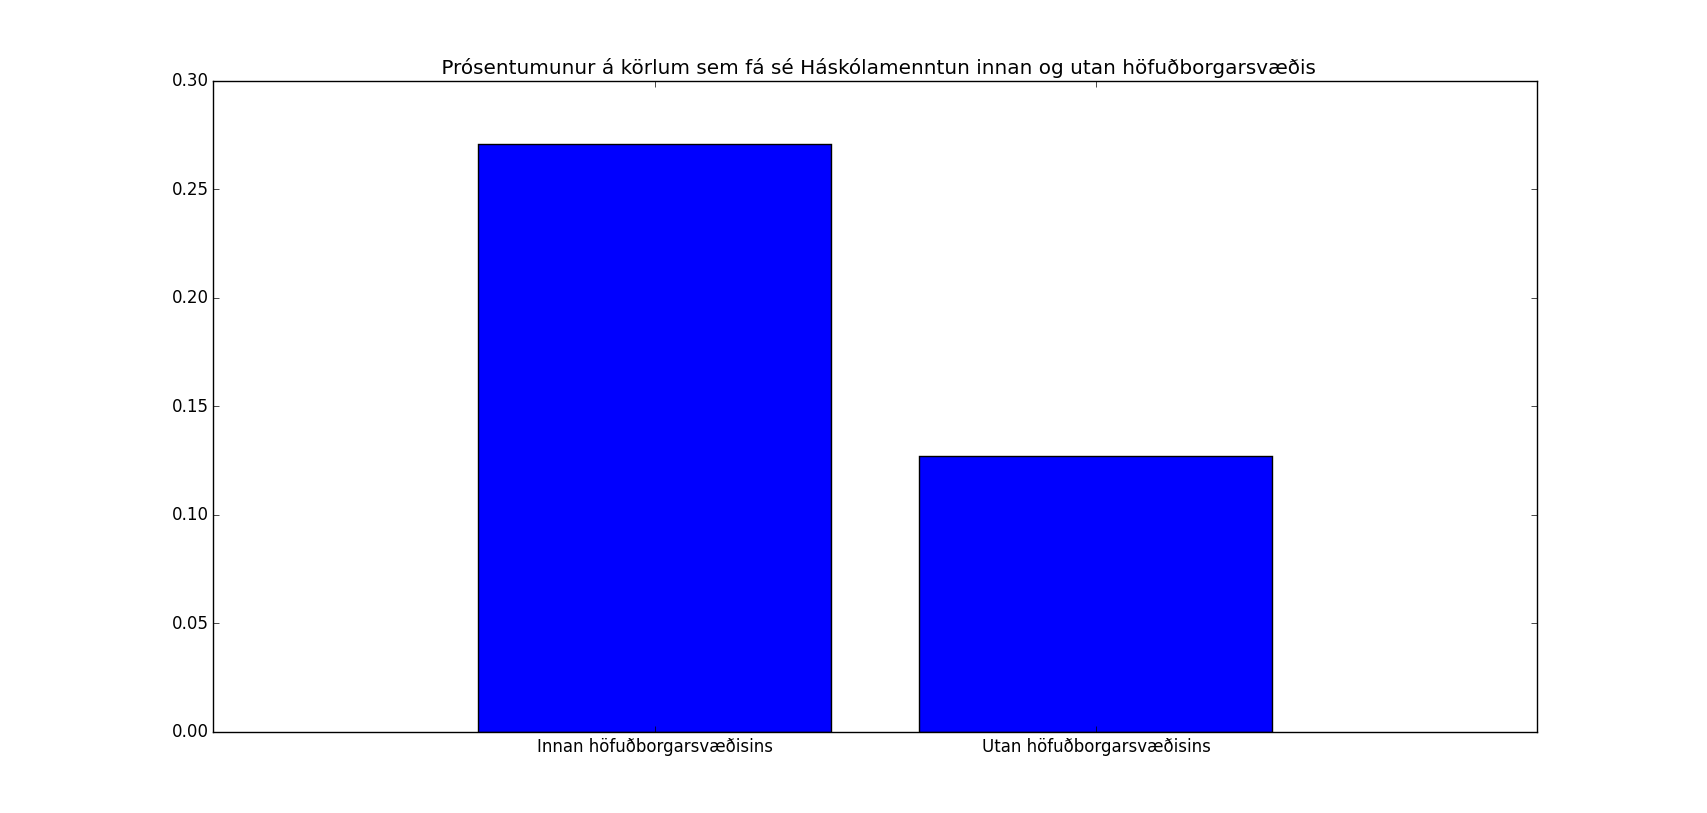
\includegraphics[width=\textwidth]{../graphics/Haskolamentun_karlar_innan_utan_hs.png}
	\caption{Modular dependency diagram for the electrical circuit \label{fig:menntukarla}}
\end{figure}

\begin{figure}
	\centering 
	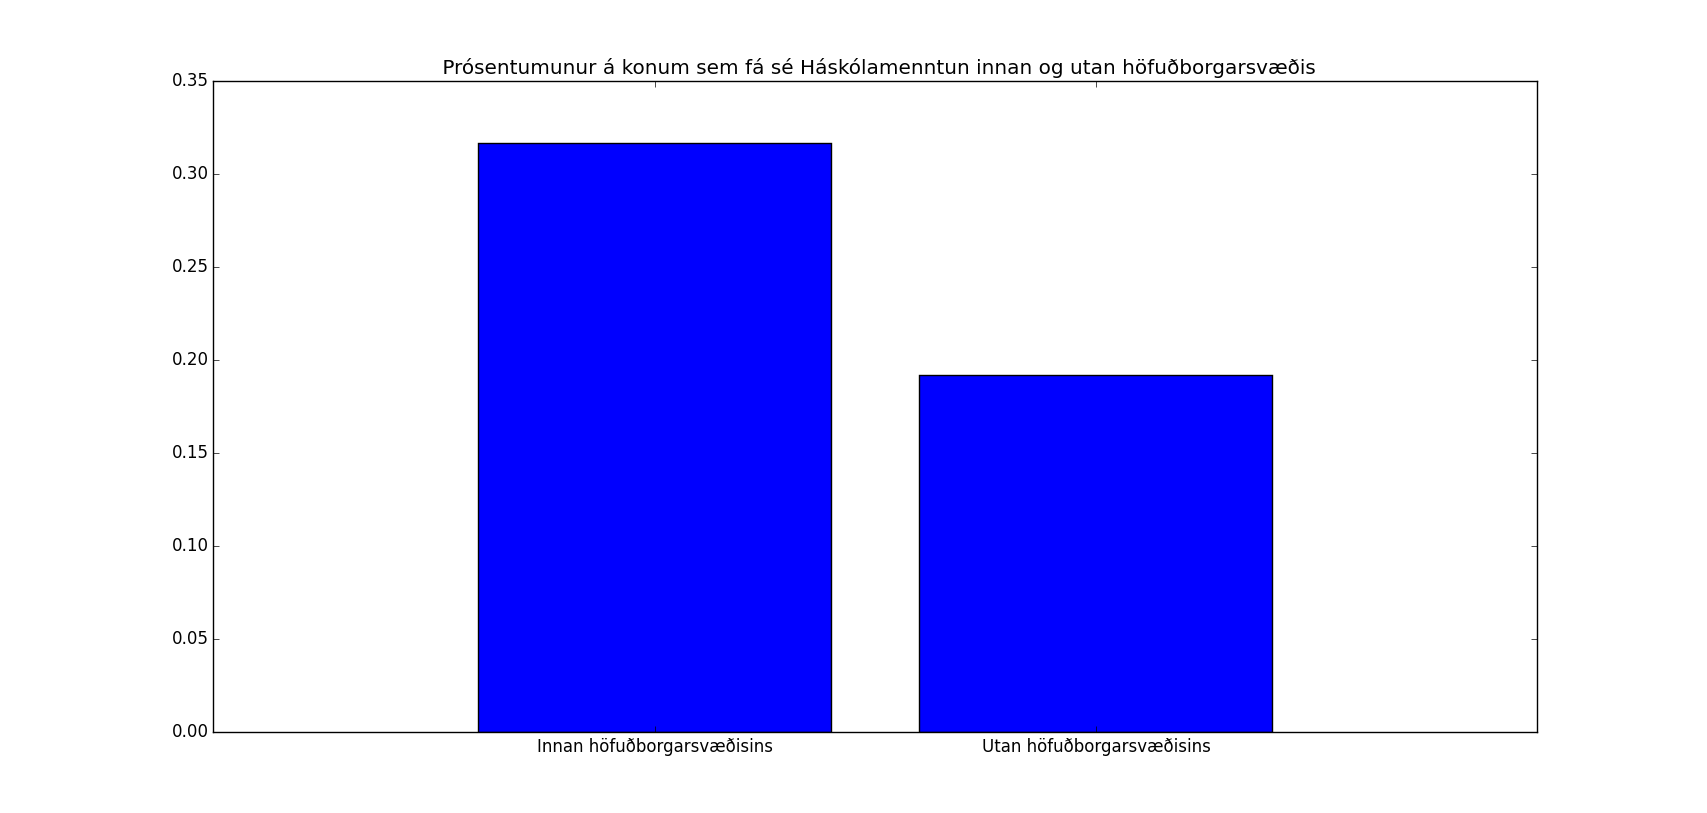
\includegraphics[width=\textwidth]{../graphics/Haskolamentun_konur_innan_utan_hs.png}
	\caption{Modular dependency diagram for the electrical circuit \label{fig:menntunkonur}}
\end{figure}

\begin{figure}
	\centering 
	\includegraphics[width=\textwidth]{../graphics/Heildar_laun.png}
	\caption{Modular dependency diagram for the electrical circuit \label{fig:heildarlaun}}
\end{figure}

\begin{figure}
	\centering 
	\includegraphics[width=\textwidth]{../graphics/Heildar_laun_og_haskolamentun.png}
	\caption{Modular dependency diagram for the electrical circuit \label{fig:heildarhask}}
\end{figure}

\begin{figure}
	\centering 
	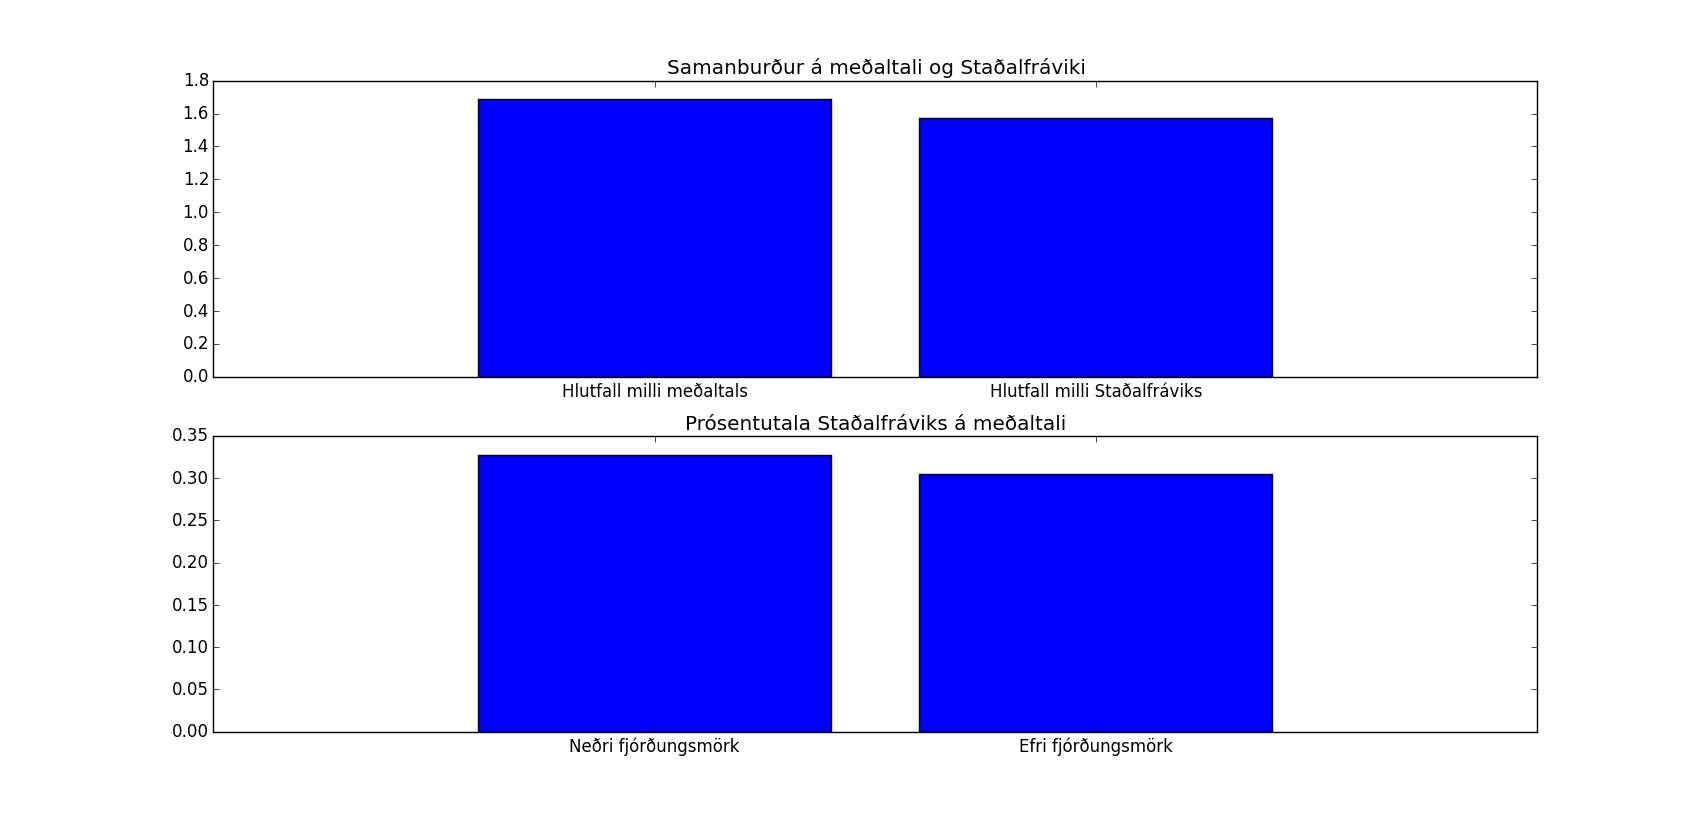
\includegraphics[width=\textwidth]{../graphics/medaltal_stadalfravik_menntun_utan_innan_hs.png}
	\caption{Modular dependency diagram for the electrical circuit \label{fig:stdhs}}
\end{figure}

\begin{figure}
	\centering 
	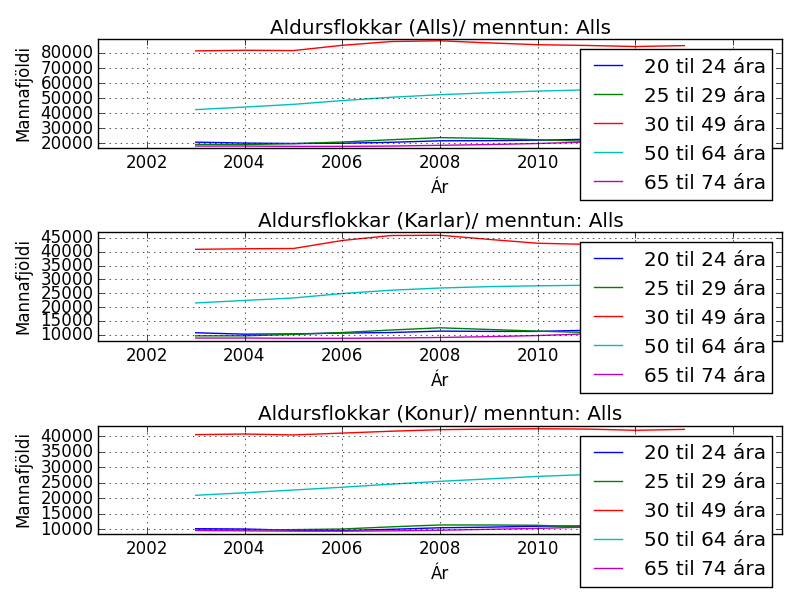
\includegraphics[width=\textwidth]{../graphics/mentun_aldrusflokkar_alls.png}
	\caption{Aldurflokkar / menntun: Alls \label{fig:menntunall}}
\end{figure}

\begin{figure}
	\centering 
	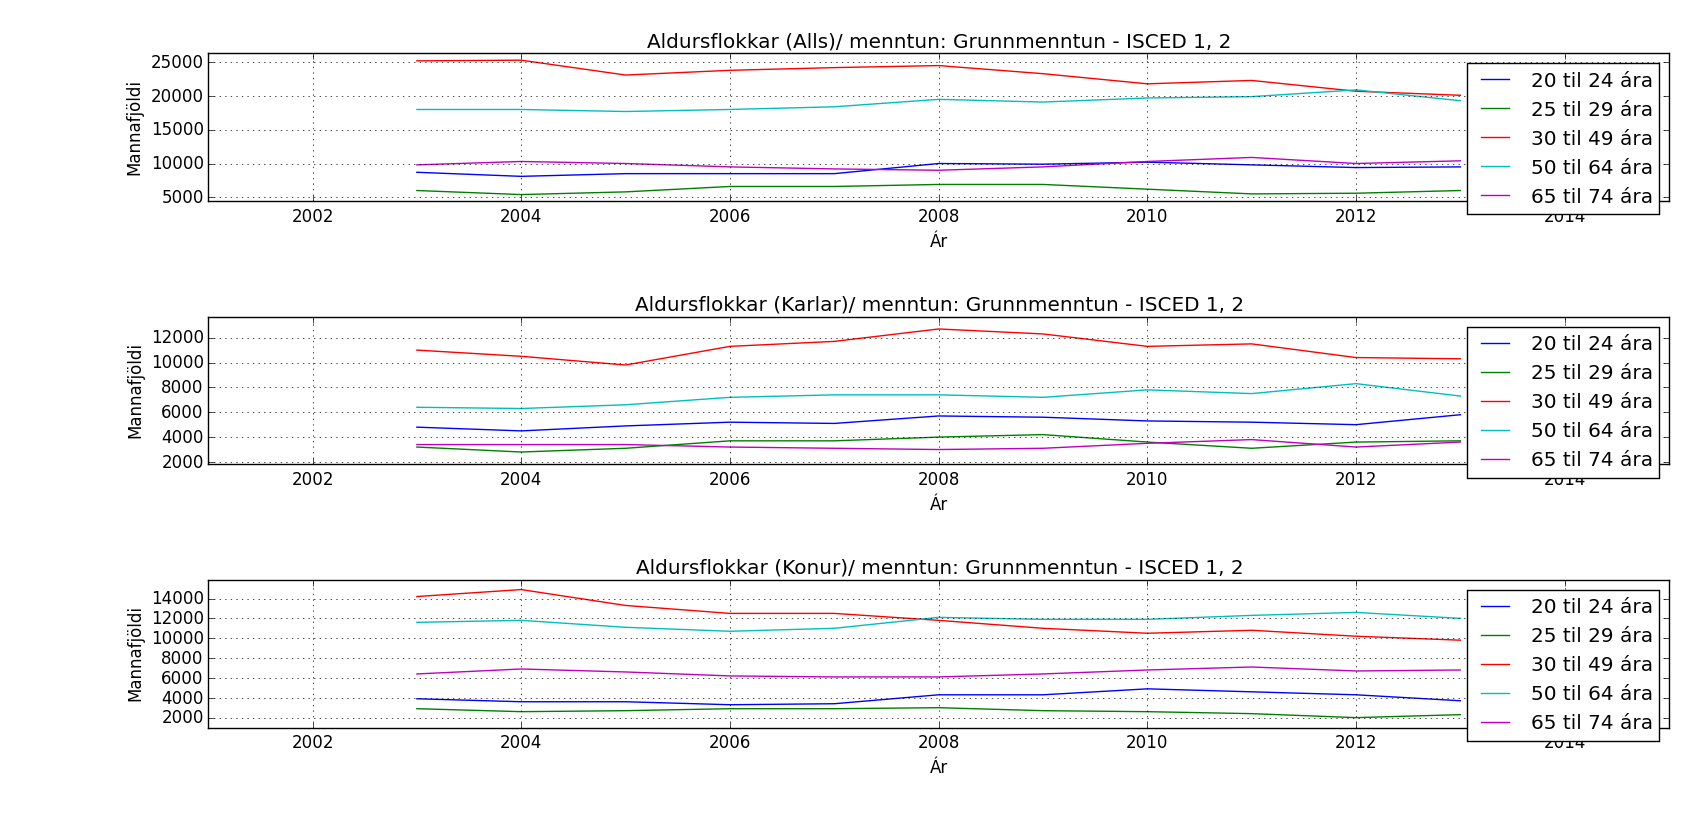
\includegraphics[width=\textwidth]{../graphics/mentun_aldrusflokkar_grunnmenntun.png}
	\caption{Aldurflokkar / menntun: Grunn- \label{fig:menntungrunn}}
\end{figure}

\begin{figure}
	\centering 
	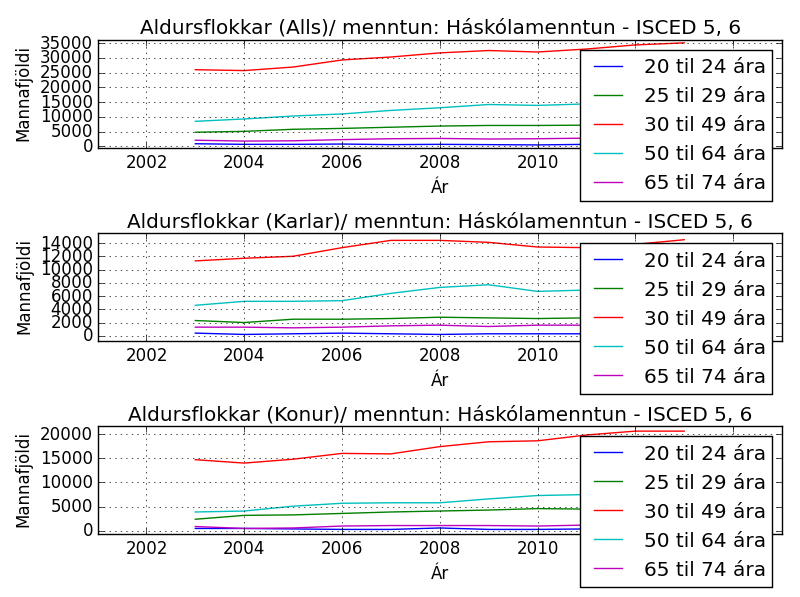
\includegraphics[width=\textwidth]{../graphics/mentun_aldrusflokkar_haskolamenntun.png}
	\caption{Aldurflokkar / menntun: Háskóla- \label{fig:menntunhs}}
\end{figure}

\begin{figure}
	\centering 
	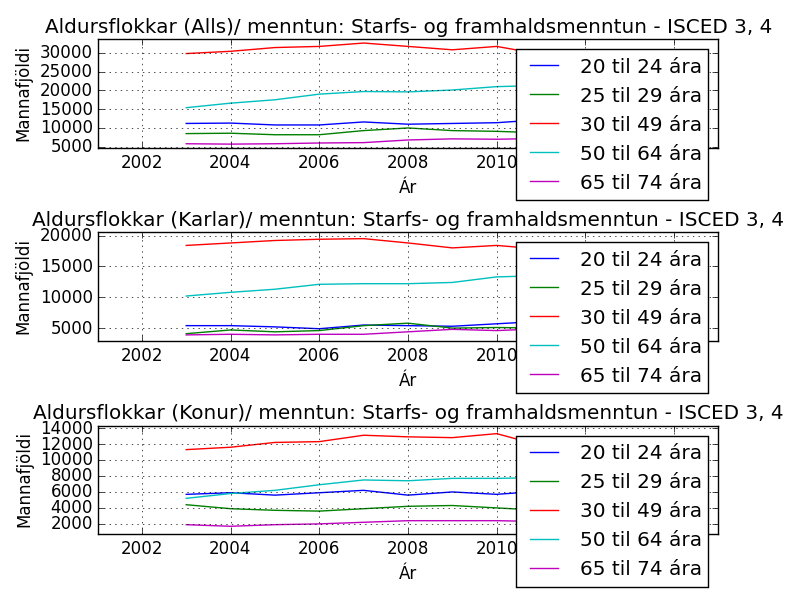
\includegraphics[width=\textwidth]{../graphics/mentun_aldrusflokkar_starfs_og_framhaldsmenntun.png}
	\caption{Aldurflokkar / menntun: Framhalds- Alls \label{fig:menntunfram}}
\end{figure}

\begin{figure}
	\centering 
	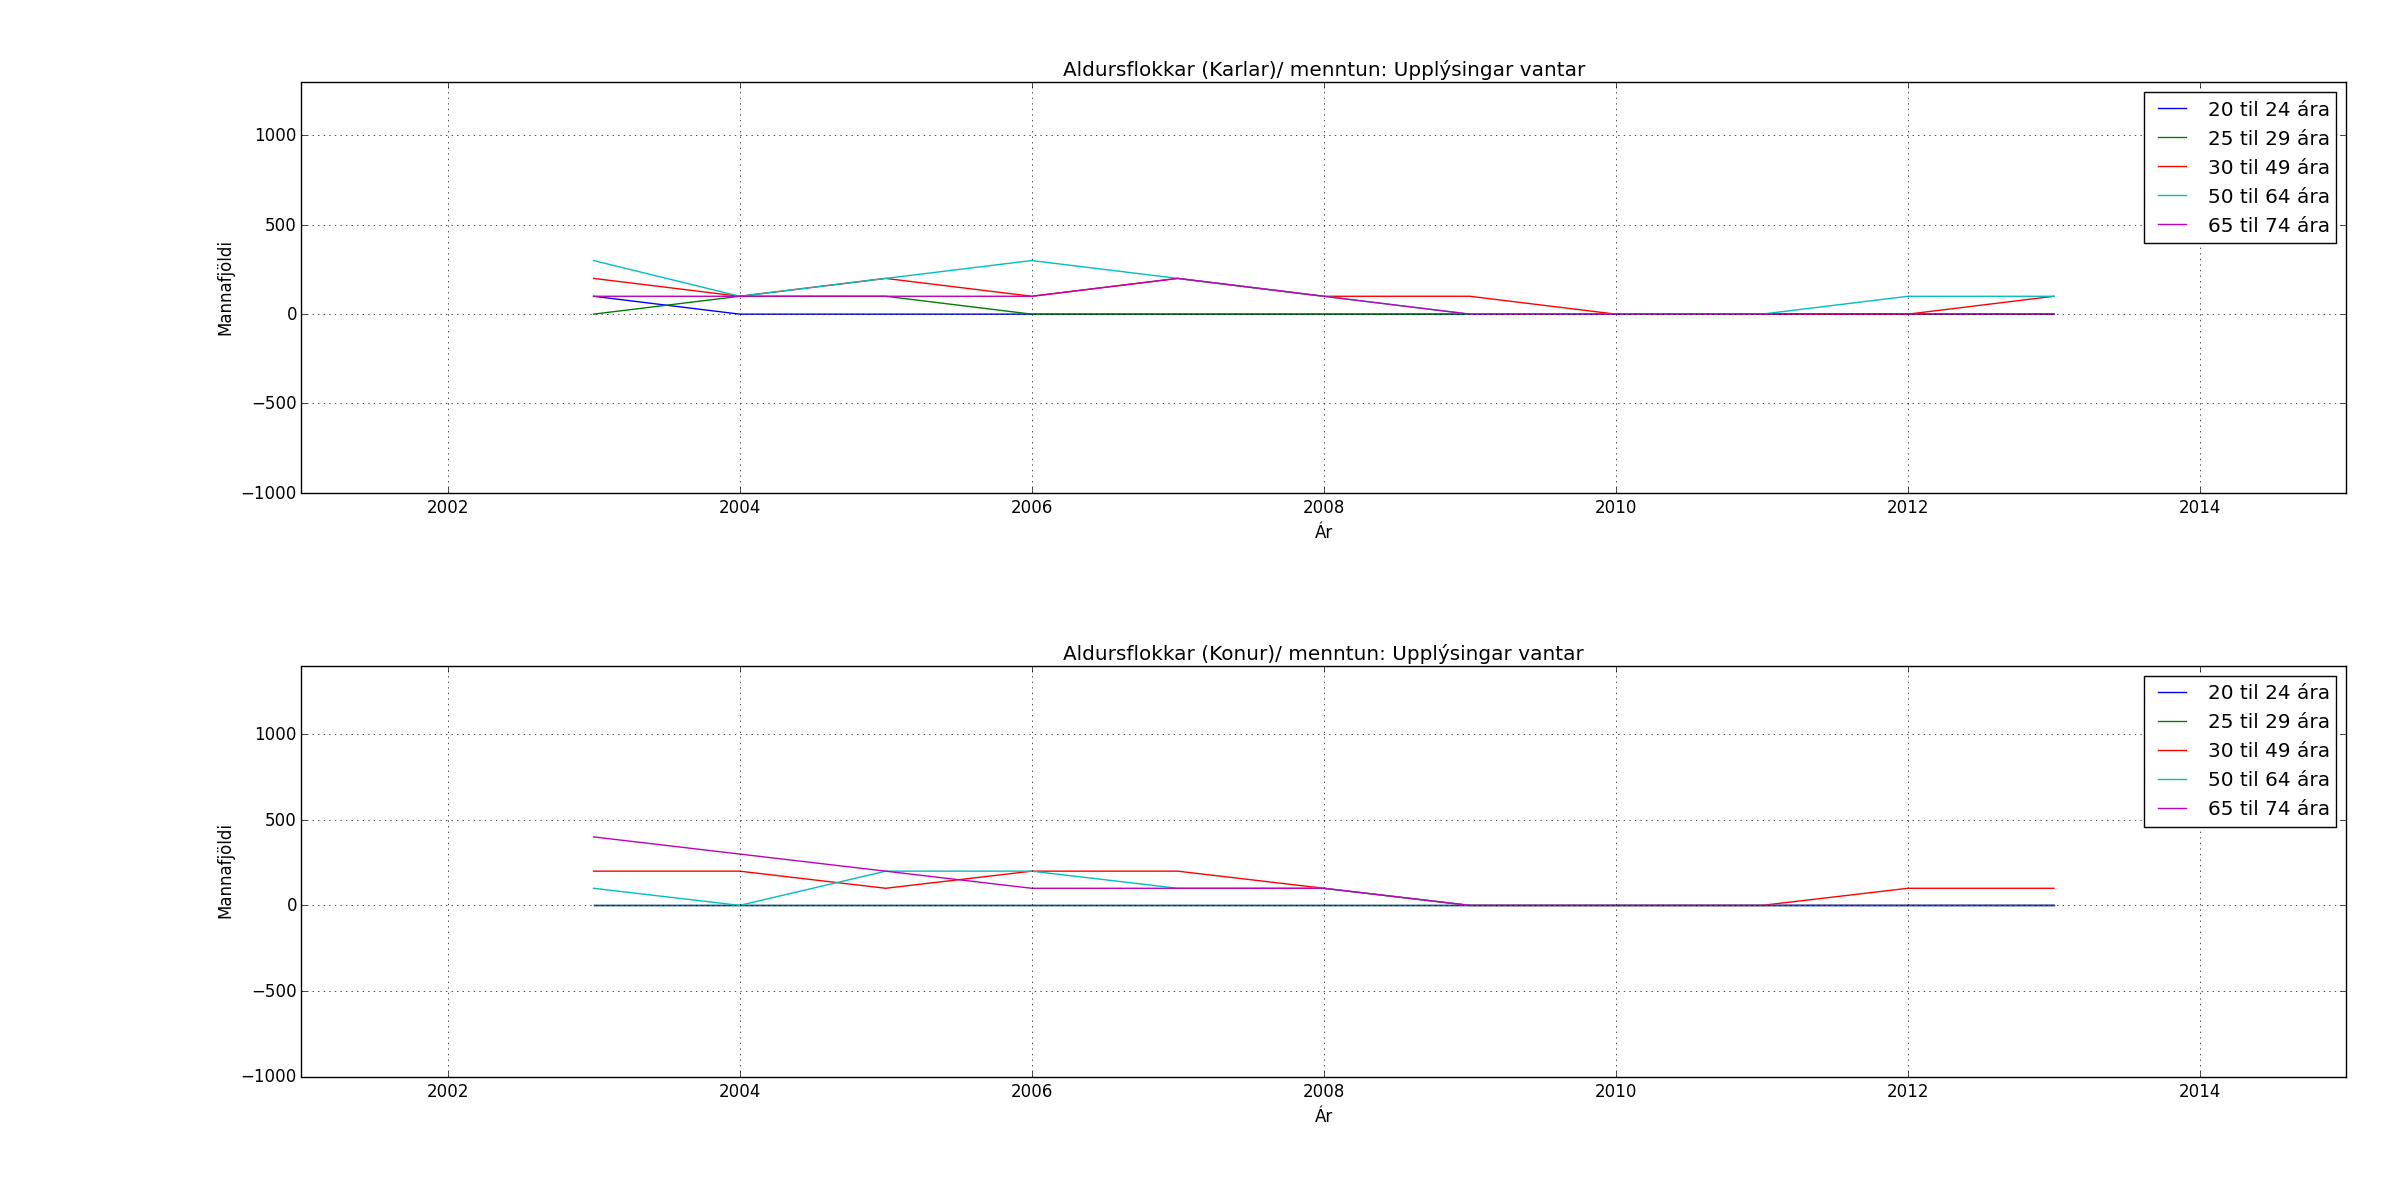
\includegraphics[width=\textwidth]{../graphics/mentun_aldrusflokkar_upplysingar_vantar.png}
	\caption{Aldurflokkar / menntun: Upplýsingar vantar \label{fig:menntunvantar}}
\end{figure}

\begin{figure}
	\centering 
	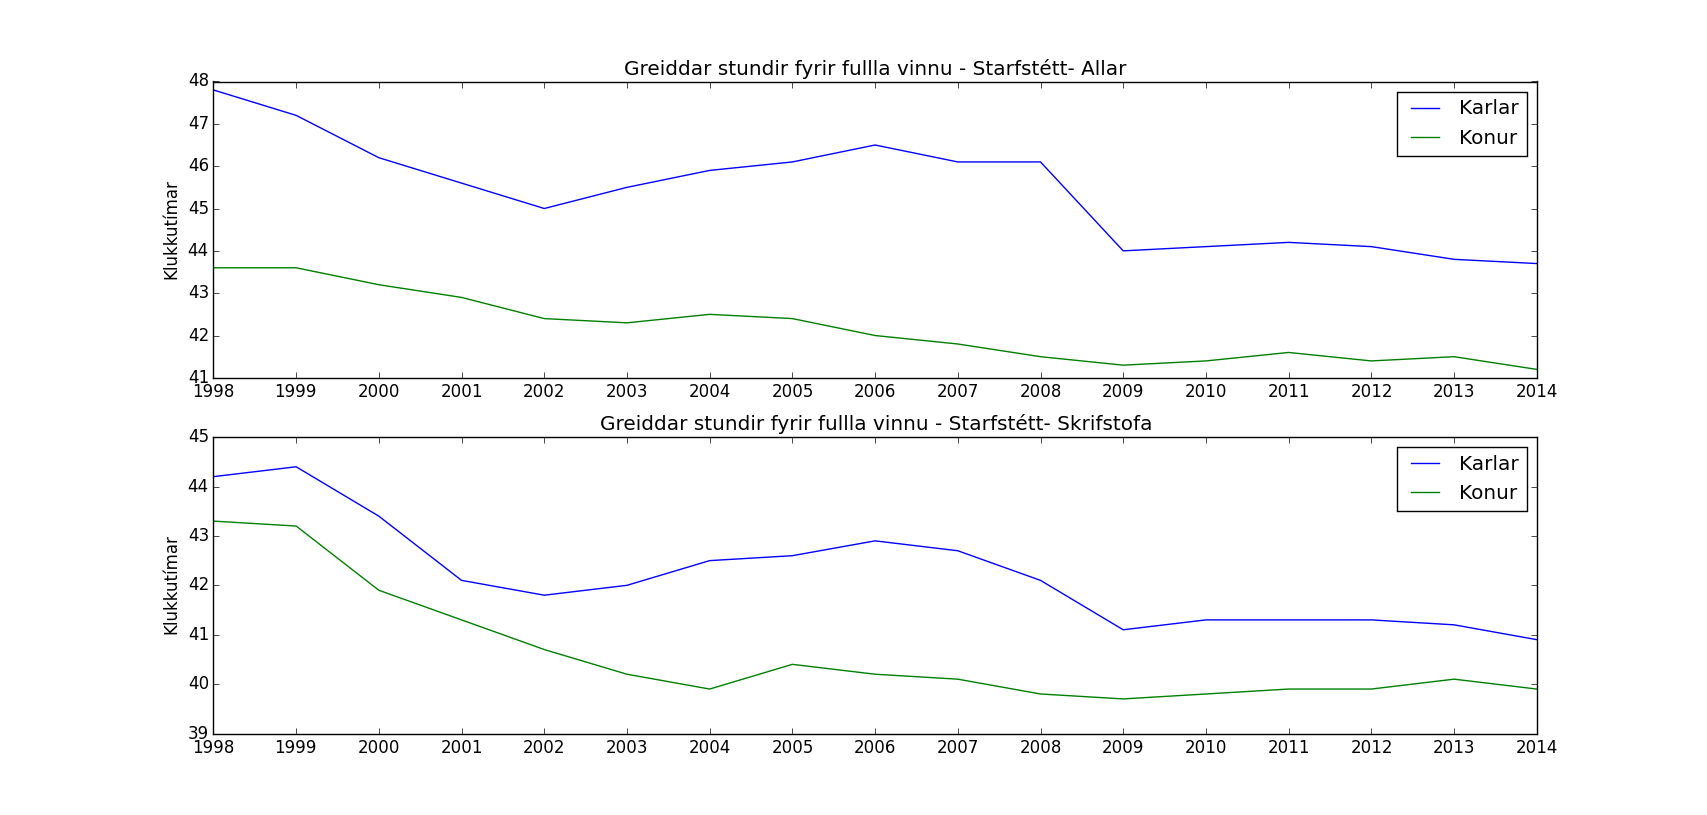
\includegraphics[width=\textwidth]{../graphics/unnir_timar1.png}
	\caption{Modular dependency diagram for the electrical circuit \label{fig:unnirtimar1}}
\end{figure}

\begin{figure}
	\centering 
	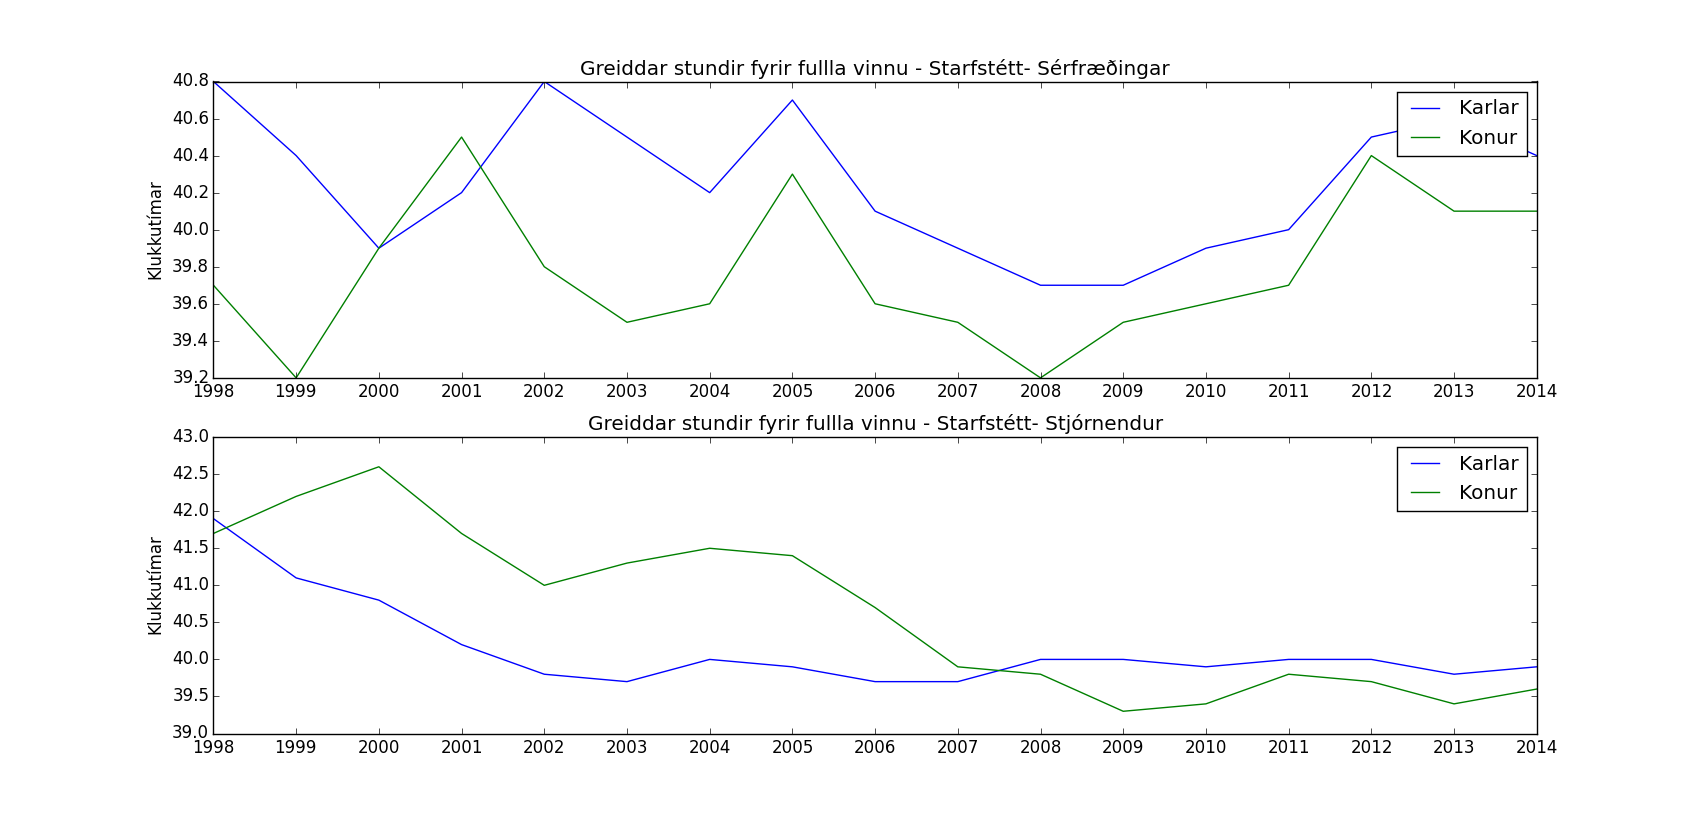
\includegraphics[width=\textwidth]{../graphics/unnir_timar2.png}
	\caption{Modular dependency diagram for the electrical circuit \label{fig:unnirtimar2}}
\end{figure}

%
\printbibliography
\end{document} % this tells the compiler that we are done

% These are variables for the editor Emacs
%%% Local Variables: 
%%% TeX-command-BibTeX: biber
%%% mode: latex
%%% TeX-master: t
%%% End:
